%! Author = Omar Iskandarani
%! Date = 2/1/2026
%! Affiliation = Independent Researcher, Groningen, The Netherlands
%! License = © 2025 Omar Iskandarani. All rights reserved. This manuscript is made available for academic reading and citation only. No republication, redistribution, or derivative works are permitted without explicit written permission from the author. Contact: info@omariskandarani.com
%! ORCID = 0009-0006-1686-3961
%! DOI = 10.5281/zenodo.xxx

\newcommand{\paperdoi}{10.5281/zenodo.xxx}
\newcommand{\papertitle}{A Variational Principle for Phase-Quantized Mesoscopic Quantum Systems}

%=========================================
% % PREAMBLE, PACKAGES AND DOCUMENT CONFIGURATION
%=========================================
\documentclass[11pt]{article}
\usepackage{amsmath,amssymb,amsfonts,bm}
\usepackage{siunitx}
\usepackage[hidelinks]{hyperref}
\usepackage[a4paper,margin=1in]{geometry}
\usepackage[T1]{fontenc}
\usepackage[utf8]{inputenc}
\usepackage{graphicx}
\usepackage{tikz}
\usepackage{pgfplots}
\pgfplotsset{compat=1.18}


\newcommand{\titlepageOpen}{
    \begin{titlepage}
        \thispagestyle{empty}  \centering
        \Large \bfseries \papertitle \par \vspace{1cm}
        {\Large \itshape \textbf{Omar Iskandarani}\textsuperscript{\textbf{*}} \par} \vspace{0.5cm}
        {\today \par}  \vspace{0.5cm}
}

\newcommand{\titlepageClose}{
        \vfill \raggedright \null
        \begin{picture}(0,0)
            \put(0,-45){  % Shift 200pt left, 40pt down
                \begin{minipage}[b]{0.7\textwidth} \footnotesize
                    \renewcommand{\arraystretch}{1.0} \noindent\rule{\textwidth}{0.4pt} \\[0.5em]
                    \textsuperscript{\textbf{*}} Independent Researcher, Groningen, The Netherlands \\
                    Email: \texttt{info@omariskandarani.com} \\
                    ORCID: \texttt{\href{https://orcid.org/0009-0006-1686-3961}{0009-0006-1686-3961}} \\
                    DOI: \href{https://doi.org/\paperdoi}{\paperdoi}
                \end{minipage}
            }
        \end{picture}
    \end{titlepage}
}
%=========================================
% Start Document - Title Page
%=========================================
\begin{document}
    \titlepageOpen
    \begin{abstract}
        Quantum systems described as ``giant atoms''—including Rydberg atoms, semiconductor quantum dots, and superconducting qubits—are traditionally treated using distinct Hamiltonian frameworks tailored to their microscopic realization. In this work we show that these systems admit a common description based on a single variational quantization principle, in which discrete spectra arise from phase closure under an effective energy functional depending on a characteristic coherence scale. The resulting formulation reproduces hydrogenic $1/n^2$ spectra, confined-dot level scalings, and Josephson-phase quantization within a unified structure.
        As a consequence, we identify a phenomenological class of orientation-dependent frequency corrections that are not excluded by standard symmetry considerations at mesoscopic coherence scales and are testable with existing spectroscopic and interferometric techniques.
    The results provide a scale-agnostic perspective on quantum quantization and suggest new precision tests of fundamental symmetries in macroscopic coherent quantum systems.
    \end{abstract}
    \titlepageClose




    \section{Introduction}

        Quantum mechanics successfully describes physical systems across an extraordinary range of length scales, from atomic orbitals to macroscopic superconducting circuits. Despite this universality, the theoretical descriptions employed for different quantum platforms often appear structurally unrelated. Atomic systems are treated using Schr\"odinger or Dirac equations with Coulombic binding potentials, semiconductor quantum dots are modeled as particles in externally imposed confinement potentials, and superconducting qubits are described by effective phase Hamiltonians derived from Josephson junction physics.

        In recent years, advances in experimental control have produced quantum systems whose spatial extent, coherence length, or effective mass differs by orders of magnitude from that of natural atoms, motivating the informal notion of ``giant atoms.'' Examples include high-principal-quantum-number Rydberg states, lithographically defined quantum dots, and superconducting qubits whose dynamical variables correspond to collective electronic phases. These systems exhibit discrete energy spectra and coherent quantum dynamics, yet interpolate between traditionally distinct microscopic and macroscopic regimes.

        This diversity raises a natural structural question: to what extent is quantum discretization tied to the microscopic details of a system, and to what extent does it follow from more general constraints associated with coherence and phase closure? While effective Hamiltonians are routinely constructed for each platform, comparatively little attention has been paid to whether a single variational principle underlies their quantization across scales.

        In this article, we show that a broad class of ``giant atom'' systems can be described by a unified variational quantization framework in which discrete energy levels arise from an extremization principle involving a characteristic coherence scale and an integer phase index. Without introducing new degrees of freedom or modifying standard quantum postulates, this approach reproduces the known spectral scalings of hydrogenic atoms, confined quantum dots, and superconducting qubits within a common mathematical structure.

        Beyond unification, the framework reveals a previously underexplored phenomenological consequence: at sufficiently large coherence scales, additional orientation-dependent frequency corrections are generically allowed by symmetry and are not forbidden by standard low-energy quantum mechanics. These corrections are parametrically small but experimentally accessible in precision measurements using mesoscopic quantum systems, such as differential qubit spectroscopy or high-resolution Rydberg interferometry.

        The paper is organized as follows. In Sec.~II we introduce the unified variational quantization functional and derive its general properties. Sections~III--V apply the framework to hydrogenic, confined, and Josephson-phase systems, respectively, demonstrating explicit agreement with established results. In Sec.~VI we discuss the phenomenological implications of orientation-dependent frequency shifts and propose experimental strategies for their detection. We conclude in Sec.~VII with a discussion of the broader implications for scale-independent quantum structure and precision tests of fundamental symmetries.

    \section{Unified Variational Quantization Framework}

        We consider quantum systems characterized by a single dominant coherence scale $R$ and a globally well-defined phase variable. Such systems include atomic orbitals with extended wavefunctions, confined electronic states in mesoscopic structures, and collective phase degrees of freedom in superconducting circuits. Rather than specifying microscopic dynamics \emph{a priori}, we focus on the minimal structural requirements for spectral discreteness under coherent phase evolution.

        \subsection{Phase Closure and Integer Quantization}

            For a coherent quantum configuration, physical admissibility requires that the total accumulated phase around a closed cycle be single-valued. This condition implies the existence of an integer-valued index $n\in\mathbb{Z}_{\geq 1}$ labeling distinct stationary configurations. Importantly, this integer does not depend on the microscopic realization of the system, but only on the existence of a closed phase trajectory.

            We assume that the energetic cost associated with phase variation scales inversely with the square of a characteristic coherence length $R$, reflecting the generic structure of gradient or kinetic terms in effective quantum Hamiltonians. To leading order, this contribution may be written as
            \begin{equation}
                E_{\mathrm{phase}}(n,R)=\frac{A\,n^2}{R^2},
            \end{equation}
            where $A$ is a positive system-dependent constant with dimensions of energy times length squared. This form encompasses, for example, orbital kinetic energy in atomic systems, confinement-induced level spacing in quantum dots, and charging energy contributions in superconducting circuits.

            \paragraph{Robustness of the quadratic phase term.}
            The quadratic dependence of the phase-related energy on the integer index
            $n$ represents the leading-order symmetry-allowed contribution consistent
            with phase periodicity and dimensional analysis. In strongly non-linear
            or strongly interacting mesoscopic systems, higher-order or non-quadratic
            corrections may arise. Such terms modify quantitative level spacings but
            do not alter the existence of discrete stationary states or the unifying
            variational mechanism at leading order.

        \subsection{Effective Binding and Confinement}

            In addition to phase-related energy costs, coherent quantum systems are stabilized by binding or confinement mechanisms that depend on the same characteristic scale $R$. We represent these effects by a general effective potential $U(R)$, whose functional form encodes the physical origin of confinement without altering the quantization mechanism itself.

            The total effective energy functional is thus taken to be
            \begin{equation}
                E_n(R)=\frac{A\,n^2}{R^2}+U(R).
                \label{eq:master-functional}
            \end{equation}

            Equation~(\ref{eq:master-functional}) constitutes the central variational object of this work. Stationary quantum states correspond to extrema of $E_n(R)$ with respect to $R$ at fixed integer $n$,
            \begin{equation}
                \left.\frac{\partial E_n}{\partial R}\right|_{n}=0,
                \label{eq:variational-condition}
            \end{equation}
            with stability determined by the second derivative.

            \paragraph{Effective-theory status of parameters.}
            The coefficients $A$ and the functional form of $U(R)$ are treated here as
            effective low-energy inputs, analogous to effective mass parameters,
            stiffness coefficients, or coupling energies in standard condensed-matter
            and circuit-QED Hamiltonians. Their microscopic origin is system-specific
            and lies outside the scope of the present structural analysis. The role of
            the variational framework is not to predict these parameters, but to show
            that once they exist, their competition uniquely determines the scaling
            structure of the discrete spectrum.

            \begin{figure}[t]
                \centering
                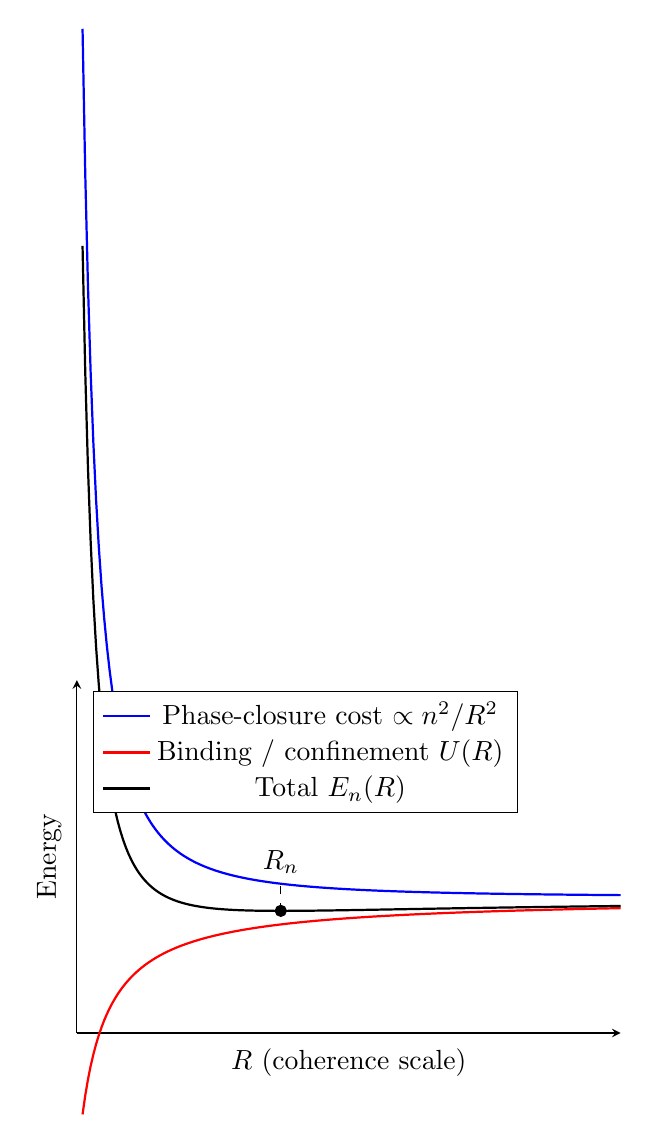
\begin{tikzpicture}
                    \begin{axis}[
                        width=0.7\linewidth,
                    height=0.5\linewidth,
                    axis lines=left,
                    xlabel={$R$ (coherence scale)},
                    ylabel={Energy},
                    xmin=0.2, xmax=5,
                    ymin=-2.5, ymax=4,
                    xtick=\empty,
                    ytick=\empty,
                    domain=0.25:5,
                    samples=200,
                    legend style={at={(0.03,0.97)},anchor=north west},
                    clip=false
                    ]

% Phase-closure term ~ n^2 / R^2
                        \addplot[blue, thick] {1/x^2};
                        \addlegendentry{Phase-closure cost $\propto n^2/R^2$}

% Confinement / binding potential (generic)
                        \addplot[red, thick] {-1/x};
                        \addlegendentry{Binding / confinement $U(R)$}

% Total energy
                        \addplot[black, thick] {1/x^2 - 1/x};
                        \addlegendentry{Total $E_n(R)$}

% Minimum point (schematic)
                        \addplot[mark=*, black] coordinates {(2, -0.25)};
                        \draw[dashed] (axis cs:2,-0.25) -- (axis cs:2,0.2);

                        \node[anchor=south] at (axis cs:2,0.25) {$R_n$};

                    \end{axis}
                \end{tikzpicture}

                \caption{Schematic illustration of the variational balance underlying
                phase-quantized coherent systems. The phase-closure contribution penalizes
                large coherence scales, while the binding or confinement potential stabilizes
                the system. Discrete stationary states correspond to extrema of the total
                effective energy functional $E_n(R)$.}
                \label{fig:phase-balance}
            \end{figure}


    \subsection{General Properties of the Variational Spectrum}

            Several general observations follow immediately from Eqs.~(\ref{eq:master-functional})--(\ref{eq:variational-condition}):

            \begin{enumerate}
                \item Discrete spectra arise solely from the integer-valued phase index $n$, independent of the detailed form of $U(R)$.
                \item The scaling of energy levels with $n$ is determined by the competition between the universal phase term $\propto n^2/R^2$ and the specific confinement mechanism encoded in $U(R)$.
                \item Systems with parametrically large coherence scales naturally exhibit dense level spacings without requiring a classical limit or semiclassical approximation.
            \end{enumerate}

            These features suggest that quantization in a wide class of ``giant atom'' systems may be understood as a geometric consequence of phase closure rather than as a property tied to microscopic length scales.

            In the following sections, we demonstrate how Eq.~(\ref{eq:master-functional}) reproduces the established spectra of hydrogenic atoms, confined quantum dots, and superconducting qubits for appropriate choices of $U(R)$, while maintaining a unified mathematical structure across all cases.

            \paragraph{Domain of applicability.}
            The present framework applies when a quantum system is characterized by a
            single dominant coherence scale and a globally well-defined phase variable.
            At sufficiently small length scales, or in regimes where multiple competing
            coherence lengths are present, a full microscopic wave-mechanical description
            is required. The variational formulation should therefore be understood as
            an effective organizational principle rather than a replacement for
            microscopic quantum dynamics.

    \section{Hydrogenic and Rydberg Systems}

        Hydrogenic atoms provide the canonical example of quantum discretization and therefore constitute a natural first test of the variational framework introduced in Sec.~II. In the standard treatment, bound states arise from solutions of the Schr\"odinger equation with a Coulomb potential, yielding the well-known $1/n^2$ energy spectrum. Here we show that the same scaling emerges directly from the unified variational functional without explicit reference to wave equations or operator formalism.

        \subsection{Effective Functional for Coulombic Binding}

            For a single-electron atom with nuclear charge $Z$, the dominant binding interaction is Coulombic. At the level of an effective radial description, the corresponding potential energy scales inversely with the characteristic orbital radius $R$. We therefore take
            \begin{equation}
                U(R) = -\frac{B}{R},
                \label{eq:coulomb-potential}
            \end{equation}
            where $B>0$ encodes the effective coupling strength, proportional to $Z e^2$ in conventional notation.

            Substituting Eq.~(\ref{eq:coulomb-potential}) into the master functional,
            \begin{equation}
                E_n(R)=\frac{A n^2}{R^2}-\frac{B}{R},
                \label{eq:hydrogen-functional}
            \end{equation}
            we obtain a one-parameter family of energy curves labeled by the integer phase index $n$.

        \subsection{Variational Extremum and Spectral Scaling}

            Stationary states correspond to extrema of $E_n(R)$ with respect to $R$ at fixed $n$,
            \begin{equation}
                \frac{\partial E_n}{\partial R}
                = -\frac{2A n^2}{R^3}+\frac{B}{R^2}=0.
            \end{equation}
            Solving for the extremal radius yields
            \begin{equation}
                R_n = \frac{2A}{B}\,n^2.
                \label{eq:rydberg-radius}
            \end{equation}

            Substituting Eq.~(\ref{eq:rydberg-radius}) back into Eq.~(\ref{eq:hydrogen-functional}) gives the energy spectrum
            \begin{equation}
                E_n = -\frac{B^2}{4A}\,\frac{1}{n^2}.
                \label{eq:rydberg-energy}
            \end{equation}

            Equations~(\ref{eq:rydberg-radius}) and (\ref{eq:rydberg-energy}) reproduce the characteristic quadratic scaling of orbital radius and inverse-square scaling of energy with the principal quantum number $n$ that define hydrogenic spectra. The specific numerical values of $A$ and $B$ may be fixed by matching to the Rydberg constant or derived from microscopic theory, but their detailed origin plays no role in establishing the scaling structure itself.

        \subsection{Rydberg States and Large Coherence Scales}

            High-principal-quantum-number Rydberg states correspond to large values of $n$ and therefore large equilibrium radii $R_n\propto n^2$. As is well known, these states exhibit small energy spacings $\Delta E\sim n^{-3}$ and long radiative lifetimes, placing them at the boundary between microscopic and mesoscopic quantum behavior \cite{Gallagher1994}.

            Within the present framework, these properties follow directly from the variational balance between the phase-related term $A n^2/R^2$ and the Coulombic binding term $-B/R$. No additional assumptions are required to describe the emergence of ``giant'' atomic states; they arise naturally as stationary solutions with parametrically large coherence scales.

            This perspective emphasizes that the qualitative features of Rydberg atoms are not tied to any specific microscopic length scale, but instead reflect the general structure of phase-quantized bound systems. In the subsequent sections, we show that this same structure governs confined mesoscopic systems and collective phase degrees of freedom in superconducting circuits.

        \subsection*{Intermezzo: Relation to Semiclassical and Bohr-Type Arguments}

            At first sight, the variational derivation presented above may appear reminiscent of early semiclassical arguments, such as Bohr's quantization of angular momentum or WKB-type approximations. It is therefore important to clarify the conceptual status of the present framework.

            The approach adopted here does not rely on classical trajectories, action quantization, or large-quantum-number approximations. In particular, no reference is made to particle orbits, classical phase-space integrals, or correspondence-principle arguments. The integer index $n$ enters solely through the requirement of global phase closure for coherent stationary configurations, a condition that remains meaningful even in regimes where semiclassical expansions fail.

            Unlike Bohr-type models, where quantization conditions are imposed directly on classical observables \cite{Bohr1913}, the present formulation operates entirely at the level of an effective energy functional whose extremization defines stationary quantum states. The phase-related term proportional to $n^2/R^2$ is not introduced as a classical kinetic energy, but as a minimal symmetry-allowed contribution consistent with coherence and dimensional analysis, analogous to gradient terms in effective field theories.

            Similarly, the framework differs from WKB or EBK quantization schemes \cite{MaslovFedoriuk1981}, which approximate solutions of an underlying wave equation in the limit of slowly varying potentials. Here no underlying differential equation is assumed; instead, the spectral structure follows from a scale-dependent variational balance between phase quantization and binding or confinement. As a result, the derivation applies equally to microscopic atomic systems and to mesoscopic or macroscopic coherent quantum devices, where semiclassical intuition is often inapplicable.

            This distinction is essential for the unifying role of the variational functional: it provides a structural explanation for discrete spectra across disparate quantum platforms without invoking classical limits, orbit-based reasoning, or asymptotic expansions. The framework should therefore be regarded not as a semiclassical approximation, but as an effective, scale-agnostic organizational principle for coherent quantum systems.

    \section{Confined Mesoscopic Systems: Quantum Dots}

        Semiconductor quantum dots are widely regarded as artificial atoms due to their discrete energy spectra and controllable confinement properties. Unlike hydrogenic systems, where binding arises from a long-range Coulomb interaction, quantum dots are stabilized by externally imposed electrostatic or structural confinement potentials. Despite this difference, we show that their spectral properties are governed by the same variational quantization framework introduced in Sec.~II.

        \subsection{Effective Confinement Potential}

            In many experimentally relevant realizations, the low-energy dynamics of a quantum dot may be approximated by an isotropic confining potential that increases with distance from the center of the dot. A commonly used minimal model is harmonic confinement, for which the effective potential scales quadratically with the characteristic confinement length $R$ \cite{Kouwenhoven2001}:
            \begin{equation}
                U(R) = C R^2,
                \label{eq:dot-potential}
            \end{equation}
            where $C>0$ encodes the strength of the confining electrostatic or structural field.

            Substituting Eq.~(\ref{eq:dot-potential}) into the master functional yields
            \begin{equation}
                E_n(R)=\frac{A n^2}{R^2}+C R^2.
                \label{eq:dot-functional}
            \end{equation}

        \subsection{Variational Spectrum}

            The stationary condition $\partial E_n/\partial R=0$ gives
            \begin{equation}
                -\frac{2A n^2}{R^3}+2C R=0,
            \end{equation}
            which is solved by
            \begin{equation}
                R_n=\left(\frac{A}{C}\right)^{1/4}\sqrt{n}.
                \label{eq:dot-radius}
            \end{equation}

            Inserting Eq.~(\ref{eq:dot-radius}) into Eq.~(\ref{eq:dot-functional}) yields the corresponding energy spectrum,
            \begin{equation}
                E_n = 2\sqrt{A C}\,\sqrt{n}.
                \label{eq:dot-energy}
            \end{equation}

            The resulting $\sqrt{n}$ scaling reflects the balance between phase-related energy costs and external confinement, and differs qualitatively from the $1/n^2$ spectrum of hydrogenic atoms. This distinction arises solely from the form of the confining potential $U(R)$ and not from any change in the underlying quantization mechanism.

        \subsection{Relation to Standard Quantum Dot Models}

            In orthodox treatments, quantum dots are described using Schr\"odinger equations with parabolic or piecewise-defined confinement potentials, leading to discrete harmonic-oscillator-like spectra \cite{ReimannManninen2002}. The present variational formulation reproduces the same qualitative level structure while abstracting away microscopic details such as effective mass, band structure, or device geometry into the parameters $A$ and $C$.

            Importantly, the appearance of discrete energy levels is again traced to the integer-valued phase index $n$ rather than to the presence of a specific microscopic length scale. As the confinement strength $C$ is reduced, the equilibrium radius $R_n$ increases and the level spacing decreases, allowing quantum dots to smoothly interpolate between microscopic and mesoscopic regimes without loss of quantization.

        \subsection{Mesoscopic Coherence and Experimental Tunability}

            Quantum dots are distinguished by their exceptional tunability: external gate voltages allow continuous control over confinement strength, particle number, and coupling to the environment. Within the present framework, such control corresponds to systematic variation of the effective parameter $C$, enabling direct experimental access to the scaling relations in Eqs.~(\ref{eq:dot-radius}) and (\ref{eq:dot-energy}).

            This tunability makes quantum dots particularly well suited for probing subtle deviations from idealized isotropic behavior. In later sections we show that, at sufficiently large coherence scales, the unified variational framework permits small orientation-dependent frequency corrections consistent with symmetry considerations, providing a new target for precision measurements in mesoscopic quantum systems.

    \section{Collective Phase Systems: Superconducting Qubits}

        Superconducting qubits constitute a distinct class of ``artificial atoms'' in which the relevant quantum degree of freedom is not the position of a particle but a collective macroscopic phase variable. Despite their radically different physical realization, such systems exhibit discrete energy spectra, coherent superpositions, and controllable transitions, making them an essential test case for any scale-agnostic quantization framework.

        \subsection{Josephson Phase as a Quantum Degree of Freedom}

            In superconducting circuits containing Josephson junctions, the dynamical variable is the superconducting phase difference $\varphi$ across the junction. The conjugate variable is the Cooper-pair number operator, leading to an effective Hamiltonian of the form \cite{Josephson1962,Devoret2013}
            \begin{equation}
                H = 4E_C \hat{n}^2 - E_J \cos \hat{\varphi},
                \label{eq:josephson-hamiltonian}
            \end{equation}
            where $E_C$ is the charging energy and $E_J$ the Josephson coupling energy. The cosine potential gives rise to a discrete spectrum of bound phase states, which may be engineered to form qubits with varying degrees of anharmonicity.

            In contrast to atomic or confined-particle systems, the phase variable $\varphi$ is dimensionless and compact, reflecting the underlying $2\pi$ periodicity of the superconducting order parameter. Nevertheless, the emergence of discrete energy levels follows from the same requirement of global phase consistency that underlies quantization in the systems discussed in Secs.~III and IV.

        \subsection{Variational Interpretation}

            To connect superconducting qubits to the unified variational framework, we note that the Josephson Hamiltonian may be interpreted as an effective energy functional for a compact phase coordinate subject to a periodic binding potential. The charging energy term $4E_C \hat{n}^2$ penalizes rapid phase variation, playing a role analogous to the phase-gradient contribution $A n^2/R^2$ in the master functional of Eq.~(\ref{eq:master-functional}), while the Josephson term $-E_J \cos\varphi$ provides stabilization through phase locking.

            Stationary quantum states correspond to extrema of the effective phase energy landscape, subject to the requirement of $2\pi$ phase closure. Discrete spectra therefore arise without reference to particle trajectories, spatial localization, or microscopic length scales, but instead from the compactness of the phase variable and the balance between phase stiffness and binding.

        \subsection{Relation to Atomic and Mesoscopic Systems}

            The connection between superconducting qubits and atomic systems is often drawn at the level of analogy, with terms such as ``artificial atoms'' used heuristically. Within the present framework, this analogy acquires a precise structural meaning: all three classes of systems considered in this work derive their discrete spectra from a competition between a phase-quantization term and a stabilizing potential.

            In hydrogenic atoms, the stabilizing potential is Coulombic; in quantum dots, it arises from external confinement; and in superconducting qubits, it is provided by the Josephson coupling. The mathematical form of the stabilizing term differs in each case, but the underlying quantization mechanism is identical.

        \subsection{Macroscopic Coherence and Precision Sensitivity}

            Superconducting qubits are distinguished by their macroscopic coherence lengths and extreme sensitivity to external perturbations. These properties make them powerful probes of subtle symmetry-allowed corrections to effective Hamiltonians. Because the relevant phase variable is collective and globally coherent, even parametrically small frequency shifts can be resolved using modern spectroscopic and interferometric techniques \cite{Koch2007,ClarkeWilhelm2008}.

            As discussed in Sec.~VI, this sensitivity enables superconducting qubits to serve as test platforms for orientation-dependent or otherwise symmetry-breaking frequency corrections that are generically permitted within an effective low-energy description, but have not yet been systematically explored experimentally.

    \section{Orientation-Dependent Frequency Corrections}

        The unified variational framework developed in the preceding sections reproduces the established spectra of hydrogenic atoms, confined mesoscopic systems, and superconducting qubits without modification of standard quantum postulates. At the same time, it naturally motivates a class of small phenomenological corrections that become relevant when the coherence scale of a quantum system is sufficiently large.

        In this section we identify orientation-dependent frequency corrections that are generically allowed within an effective low-energy description of coherent quantum systems, and discuss their experimental observability.

        \subsection{Symmetry Considerations}

            Conventional nonrelativistic quantum mechanics assumes exact rotational invariance of isolated systems in the absence of external fields. However, at the level of effective Hamiltonians describing mesoscopic or macroscopic coherent objects, rotational symmetry need not be exact if additional background structures or weak symmetry-breaking effects are present. From a purely phenomenological standpoint, it is therefore appropriate to ask which corrections to energy levels are allowed by minimal consistency requirements, even if their microscopic origin is left unspecified.

            For a stationary quantum system characterized by a dominant transition frequency $\omega_0$, the most general leading-order correction consistent with time-reversal symmetry and analyticity may be written as
            \begin{equation}
                \omega(\mathbf{V},\hat{\mathbf{n}}) =
                \omega_0
                + \epsilon_1 \frac{\mathbf{V}^2}{c^2}
                + \epsilon_2 \frac{(\mathbf{V}\cdot\hat{\mathbf{n}})^2}{c^2}
                + \mathcal{O}\!\left(\frac{V^4}{c^4}\right),
                \label{eq:anisotropic-frequency}
            \end{equation}
            where $\mathbf{V}$ is the laboratory velocity with respect to a chosen inertial frame, $\hat{\mathbf{n}}$ is a system-specific orientation axis, and $\epsilon_{1,2}$ are phenomenological coefficients.

            The isotropic term proportional to $\mathbf{V}^2$ merely renormalizes the transition frequency and is generally unobservable in isolation. In contrast, the anisotropic term proportional to $(\mathbf{V}\cdot\hat{\mathbf{n}})^2$ leads to orientation-dependent frequency shifts that can be experimentally distinguished.

        \subsection{Relation to Existing Frameworks}

            Orientation-dependent effects of the form in Eq.~(\ref{eq:anisotropic-frequency}) are not forbidden by standard quantum mechanics, but they are typically neglected because they are expected to be extremely small for microscopic systems. Similar parametrizations appear in effective field-theory extensions of the Standard Model and in phenomenological analyses of Lorentz and rotational symmetry tests \cite{Kostelecky1995,Mattingly2005}.

            What distinguishes the present context is the focus on systems with large coherence scales, such as Rydberg atoms and superconducting qubits, where collective phase coherence amplifies sensitivity to small frequency shifts. In such systems, orientation-dependent corrections may be enhanced relative to microscopic atoms without introducing any modification of fundamental quantum principles.

        \subsection{Experimental Signatures}

            The laboratory velocity $\mathbf{V}$ relative to an inertial reference frame varies in both magnitude and direction due to the Earth's rotation and orbital motion. As a result, the anisotropic term in Eq.~(\ref{eq:anisotropic-frequency}) predicts characteristic periodic modulations of transition frequencies with sidereal and annual periods.

            Experimentally accessible signatures include:
            \begin{enumerate}
                \item Daily modulation of transition frequencies correlated with the orientation of the system relative to the Earth's rotation axis.
                \item Differential frequency shifts between two otherwise identical systems oriented along orthogonal axes.
                \item Absence of correlated shifts in control parameters sensitive only to environmental noise, enabling discrimination from systematic effects.
            \end{enumerate}

            Superconducting qubits are particularly well suited for such tests due to their long coherence times, high frequency resolution, and controllable geometry \cite{ClarkeWilhelm2008}. Rydberg atoms and confined quantum dots provide complementary platforms with distinct sources of systematic uncertainty.

            \paragraph{Order-of-magnitude sensitivity.}
            For laboratory experiments on Earth, the orbital velocity satisfies
            $V/c \sim 10^{-4}$, implying $(V/c)^2 \sim 10^{-8}$. State-of-the-art
            superconducting qubit spectroscopy routinely achieves relative frequency
            resolutions at or below the $10^{-9}$ level over experimentally relevant
            integration times. As a result, existing platforms are already sensitive
            to anisotropic coefficients $|\epsilon_2|$ at the level of $10^{-2}$--$10^{-3}$,
            with future improvements expected as coherence times and control protocols
            advance.

        \subsection{Distinguishability from Decoherence Effects}

            A key feature of the predicted corrections is their coherent and reproducible nature. Unlike decoherence or environmental noise, which typically manifests as stochastic fluctuations or irreversible loss of phase information, orientation-dependent frequency shifts would appear as deterministic, periodic signals with well-defined symmetry properties.

            This distinction enables the use of differential measurement strategies, such as Ramsey interferometry or synchronized multi-device comparisons, to isolate the effect from conventional noise sources \cite{Wineland1994}. The phenomenological parameters $\epsilon_{1,2}$ may thus be constrained or bounded using existing experimental techniques.

        \subsection{Implications}

            The existence of orientation-dependent frequency corrections consistent with Eq.~(\ref{eq:anisotropic-frequency}) would have significant implications for the interpretation of precision measurements in mesoscopic quantum systems. Conversely, null results can be used to place stringent bounds on such effects, thereby constraining a broad class of effective low-energy theories.

            Importantly, the analysis presented here does not depend on any specific microscopic model for the origin of the anisotropy. The results therefore serve as a general phenomenological benchmark for future experimental investigations of coherent quantum systems at large scales.

    \section{Discussion and Conclusions}

        In this work we have shown that a broad class of quantum systems commonly described as ``giant atoms'' admits a unified description based on a single variational quantization framework. By focusing on phase closure and a characteristic coherence scale, the approach reproduces the established spectra of hydrogenic atoms, confined mesoscopic systems such as quantum dots, and collective phase systems realized in superconducting qubits. The derivations require no modification of standard quantum postulates and introduce no new microscopic degrees of freedom.

        The central result is structural rather than dynamical: discrete quantum spectra emerge generically from the competition between a phase-related energy cost and a stabilizing potential, independent of the microscopic origin of that potential. Differences between atomic, mesoscopic, and macroscopic quantum systems are reflected solely in the functional form of the effective confinement term, while the underlying quantization mechanism remains unchanged. This perspective clarifies why systems with vastly different length scales and physical realizations nevertheless display closely analogous quantum behavior.

        Beyond unification, the framework motivates a phenomenological extension in which orientation-dependent frequency corrections are permitted at large coherence scales. These corrections are consistent with symmetry considerations and effective low-energy descriptions, yet are typically neglected in microscopic quantum systems due to their extreme smallness. Advances in experimental control and coherence now place mesoscopic quantum platforms in a regime where such effects can be meaningfully constrained or detected.

        Importantly, the analysis deliberately refrains from attributing the proposed anisotropies to any specific microscopic mechanism. The orientation-dependent terms are introduced as effective parameters, analogous to those employed in broader searches for symmetry violations or emergent background structures. As such, the present work provides a model-independent benchmark against which precision experiments may be compared.

        Several directions for future research follow naturally. On the theoretical side, it would be valuable to explore whether the variational framework can be derived systematically from coarse-grained microscopic models or effective field theories. On the experimental side, differential spectroscopy using orthogonally oriented superconducting qubits, high-principal-quantum-number Rydberg atoms, or tunable quantum dots offers a realistic path toward placing bounds on the phenomenological coefficients introduced here.

        More broadly, the results suggest that quantum discretization is best understood as a scale-agnostic consequence of coherence and phase structure, rather than as a property tied to specific microscopic constituents. As quantum systems continue to grow in size and complexity, such unifying perspectives may play an increasingly important role in organizing and interpreting experimental observations across traditionally distinct domains.


%==============================
% References
%==============================

            \begin{thebibliography}{99}

                \bibitem{Kostelecky1995}
                V.~A.~Kosteleck\'y and R.~Potting (1995),
                ``CPT and strings,''
                \emph{Physical Review D} \textbf{51}, 3923--3935.
                DOI: 10.1103/PhysRevD.51.3923.

                \bibitem{Mattingly2005}
                D.~Mattingly (2005),
                ``Modern tests of Lorentz invariance,''
                \emph{Living Reviews in Relativity} \textbf{8}, 5.
                DOI: 10.12942/lrr-2005-5.

                \bibitem{Wineland1994}
                D.~J.~Wineland \emph{et al.} (1994),
                ``Squeezed atomic states and projection noise in spectroscopy,''
                \emph{Physical Review A} \textbf{50}, 67--88.
                DOI: 10.1103/PhysRevA.50.67.


                \bibitem{Josephson1962}
                B.~D.~Josephson (1962),
                ``Possible new effects in superconductive tunnelling,''
                \emph{Physics Letters} \textbf{1}, 251--253.
                DOI: 10.1016/0031-9163(62)91369-0.

                \bibitem{Devoret2013}
                M.~H.~Devoret and R.~J.~Schoelkopf (2013),
                ``Superconducting circuits for quantum information,''
                \emph{Science} \textbf{339}, 1169--1174.
                DOI: 10.1126/science.1231930.

                \bibitem{Koch2007}
                J.~Koch \emph{et al.} (2007),
                ``Charge-insensitive qubit design derived from the Cooper pair box,''
                \emph{Physical Review A} \textbf{76}, 042319.
                DOI: 10.1103/PhysRevA.76.042319.

                \bibitem{ClarkeWilhelm2008}
                J.~Clarke and F.~K.~Wilhelm (2008),
                ``Superconducting quantum bits,''
                \emph{Nature} \textbf{453}, 1031--1042.
                DOI: 10.1038/nature07128.

                \bibitem{Kouwenhoven2001}
                L.~P.~Kouwenhoven, D.~G.~Austing, and S.~Tarucha (2001),
                ``Few-electron quantum dots,''
                \emph{Reports on Progress in Physics} \textbf{64}, 701--736.
                DOI: 10.1088/0034-4885/64/6/201.

                \bibitem{ReimannManninen2002}
                S.~M.~Reimann and M.~Manninen (2002),
                ``Electronic structure of quantum dots,''
                \emph{Reviews of Modern Physics} \textbf{74}, 1283--1342.
                DOI: 10.1103/RevModPhys.74.1283.

                \bibitem{Bohr1913}
            N.~Bohr (1913),
            ``On the Constitution of Atoms and Molecules,''
            \emph{Philosophical Magazine} \textbf{26}, 1--25.

            \bibitem{BetheSalpeter1957}
            H.~A.~Bethe and E.~E.~Salpeter (1957),
            \emph{Quantum Mechanics of One- and Two-Electron Atoms},
            Springer, Berlin.
            DOI: 10.1007/978-3-642-60843-4.

            \bibitem{Gallagher1994}
            T.~F.~Gallagher (1994),
            \emph{Rydberg Atoms},
            Cambridge University Press.
            ISBN: 9780521389736.

            \bibitem{CohenTannoudji1977}
            C.~Cohen-Tannoudji, B.~Diu, F.~Lalo\"e (1977),
            \emph{Quantum Mechanics}, Vol.~1,
            Wiley, New York.
            ISBN: 9780471164328.


        \bibitem{MaslovFedoriuk1981}
        V.~P.~Maslov and M.~V.~Fedoriuk (1981),
        \emph{Semi-Classical Approximation in Quantum Mechanics},
        Reidel, Dordrecht.
        DOI: 10.1007/978-94-009-8490-0.



            \end{thebibliography}

\end{document}